% !TEX root = Eco-Model.tex
\section{Problem Background} % (fold)
\label{sec:problem_background}

\subsection{Cloud Manufacturing Ecosystem} % (fold)
\label{sub:cloud_manufacturing_ecosystem}
As an application of Networked Manufacturing, Cloud Mfg ...
\begin{figure}[htbp]
\centering
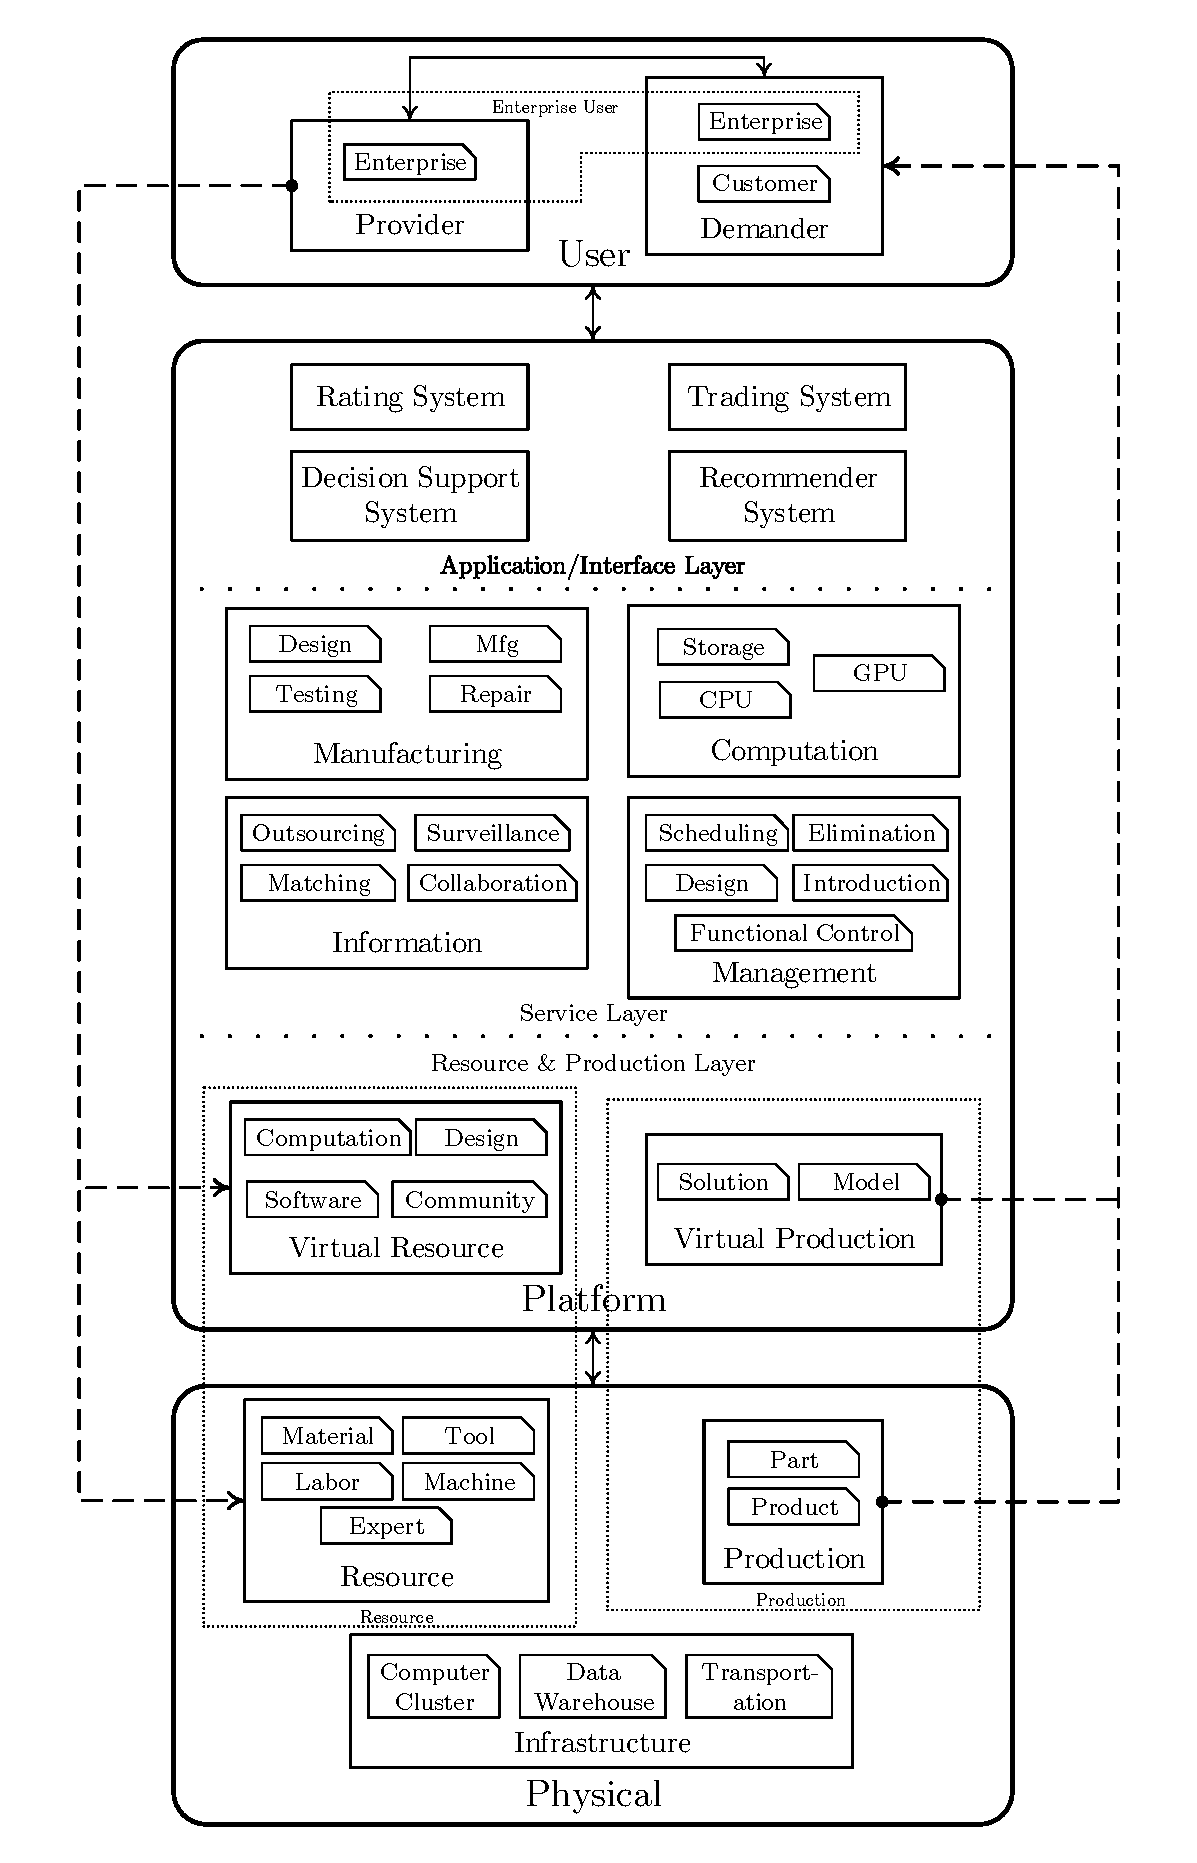
\includegraphics[scale = .6, trim = 0 15 0 0]{Cloud_Mfg_Structure.pdf}
\caption{Cloud Manufacturing Architecture with Main Flows}
\label{fig:structure}
\end{figure}





As shown in \autoref{fig:structure}, the architecture of Cloud Mfg is mainly comprised by three parts, namely User, Platform and Physical Base, some of whose subparts are connected by (material or information) flows. With the supplementary illustration in \autoref{fig:supplementary}

\begin{figure}[htbp]
\centering
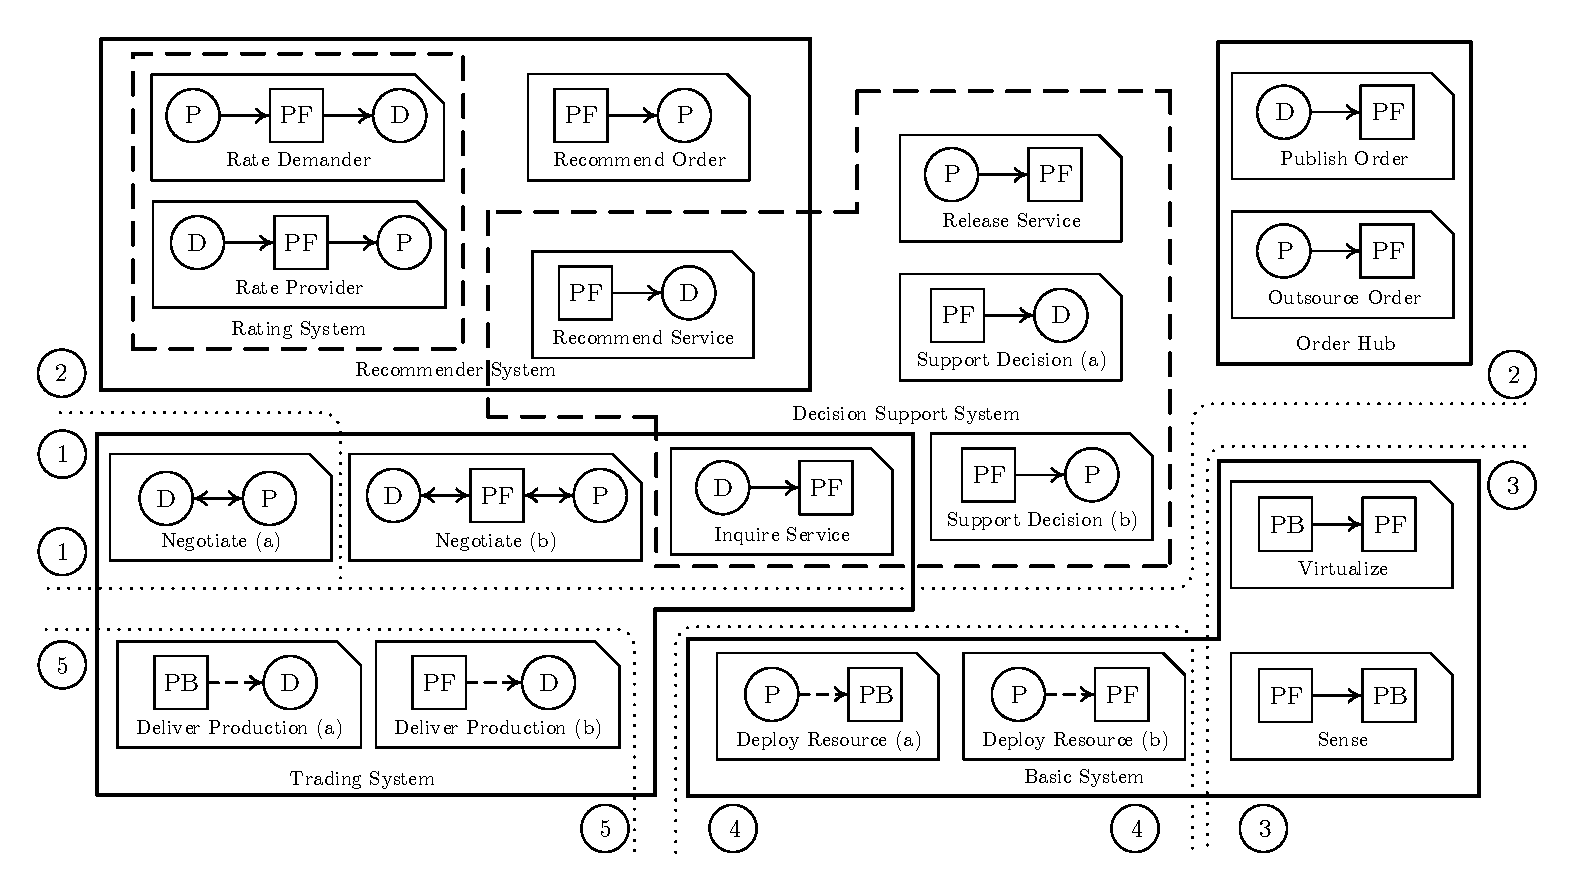
\includegraphics[scale = .6, trim = 0 15 0 0]{supplementary.pdf}
\caption{Supplementay Illustration of \autoref{fig:structure}}
\label{fig:supplementary}
\end{figure}

Modular approaches are widely used to decompose a complex system into smaller subsystems according to their functions. For example, Yang and Li (2011) divided a cloud manufacturing services management and control platform into seven functional modules such as system management module, production management module and so on

\subsubsection{Enterprise Business Mode}

\subsubsection{Resource Sharing Mechanism}

\subsubsection{Ecosystem Adjustment}

% subsection cloud_manufacturing_ecosystem (end)

\subsection{Main Copmlexity Concepts} % (fold)
\label{sub:main_copmlexity_concepts}

\subsubsection{Self-organization}

\subsubsection{Emergence}

\subsubsection{Co-evolution}

\subsubsection{Adaption}
% subsection main_copmlexity_concepts (end)

\subsection{Ecosystem Evolvement} % (fold)
\label{sub:ecosystem_evolvement}

% subsection ecosystem_evolvement (end)

\subsection{Optimal Guidance} % (fold)
\label{sub:optimal_guidance}

% subsection optimal_guidance (end)
% section problem_background (end)